\documentclass[letterpaper,12pt]{article}

\RequirePackage[hypertex]{hyperref}
    \hypersetup{colorlinks=true,urlcolor=blue,linkcolor=red}
\RequirePackage{GE05}

\newcommand{\GDP}{\mbox{\em GDP\/}}
\newcommand{\NDP}{\mbox{\em NDP\/}}
\newcommand{\GNP}{\mbox{\em GNP\/}}
\newcommand{\NX}{\mbox{\em NX\/}}
\newcommand{\NY}{\mbox{\em NY\/}}
\newcommand{\CA}{\mbox{\em CA\/}}
\newcommand{\NFA}{\mbox{\em NFA\/}}
\newcommand{\Def}{\mbox{\em Def\/}}
\newcommand{\CPI}{\mbox{\em CPI\/}}
\newcommand{\IP}{\mbox{\em IP\/}}


\def\ClassName{The Global Economy}
\def\Category{Class Notes}
\def\HeadName{Business Cycle Indicators \& Forecasting}

\begin{document}
\thispagestyle{empty}%
\Head

\centerline{\large \bf \HeadName}%
\centerline{Revised: \today}

\bigskip
If economies grow unevenly, what can we do about it? 
With luck, we can forecast these ups and downs and plan for them:
businesses can decide how many people to hire and how much to produce, 
investors can decide how to allocate their assets, 
and households can decide how much to spend. 
The good news is that forecasting is possible;  
we're not simply throwing darts at a board.  
The bad news is that it's not easy --- 
even the best forecasters are far from perfect.

This set of notes is devoted to short-term ``business cycle''
indicators ---  variables that indicate changes in the short-term 
movements in the economy --- 
and how to use them.  
In principle we could be interested in many features of
the economy:  output, inflation, interest rates, 
exchange rates, and so on. 
We'll focus on output, but the methods can easily be applied 
to other variables.   
We'll look at the US, 
but similar ideas and methods apply to any country with reliable data. 


\subsubsection*{The forecasting ``problem''}

The classic forecasting problem goes something like this:  What do we expect the value of [some
economic variable] to be $k$ periods in the future?  
Here $k$ is any period of time you like, but
we're usually interested in anything from next week to a few years in 
the future.  

\begin{figure}
    \centering
    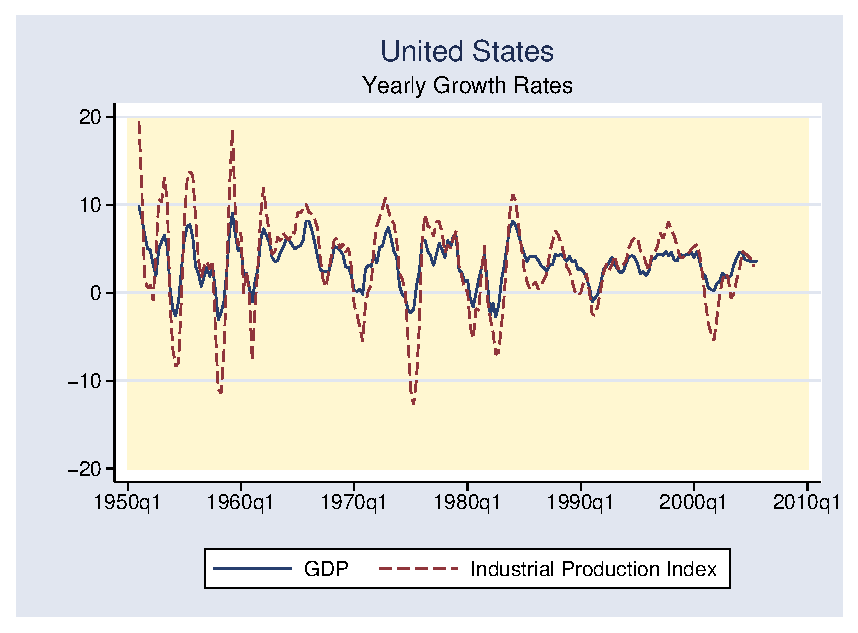
\includegraphics[scale=0.8]{us_gdp_indprod.eps}
    \caption{GDP and Industrial Production.}
    \label{fig:ip_gdp}%
\end{figure}


If we're forecasting GDP, there's an extra difficulty: we don't
know the present or the recent past, much less the future. We've
seen, for example, that fourth-quarter GDP is first reported near
the end of the following January, and even that number is a
preliminary estimate. From the perspective of mid-January, then,
we need to ``forecast'' the previous quarter.


We're going to shortcut this difficulty (somewhat) by using the
monthly Industrial Production (IP) index as a substitute for real
GDP, but the issue is a general one:  the time lag in getting data
is both an issue in its own right and a  constraint on forecasting
the future. IP measures output in manufacturing, mining, and
utilities. More important, its fluctuations are strongly
correlated with those in GDP.  You can see that in
Figure~\ref{fig:ip_gdp}, which compares year-on-year growth rates
in GDP and IP (aggregated to a quarterly frequency). You will
notice that IP is more volatile than GDP but otherwise follows its
ups and downs reasonably well.  You may also notice some
differences between them in the recent past, which have been
traced to the rising importance of services in the US economy.  In
the US, IP is reported by the Federal Reserve in the middle of the
following month.  Data for December, for example, are available in
mid-January.  Using IP therefore gives us a shorter information
lag than GDP.  In addition, the monthly frequency gives us a finer
time interval for near-term forecasting.  For both reasons, we
will focus our discussion of forecasting on IP rather than GDP,
although the same principles apply to both, as well as to other
macroeconomic and financial variables.


\subsubsection*{Properties of economic indicators}

We refer to the properties of economic indicators with 
two related sets of terms.
One set of terms describes whether the indicator's movements
tend to come before or after movements in (say) output.  
We say an indicator {\it leads\/} output if 
its ups and downs generally precede those of output, 
and {\it lags\/} output if they come after.  
An indicator whose movements are contemporaneous with those of output 
is referred to as {\it coincident\/}.
Thus the adjectives leading, lagging, and  coincident 
describe the timing of an indicator's movements relative to those of output.
Looking ahead, you might guess that leading indicators are 
most useful in forecasting.  
The stock market, for example, is a common leading indicator;
it leads output by 6-8 months, as we'll see shortly.  

A second set of terms refers to whether an indicator's movements
are positively or negatively correlated with output.
If the correlation is positive, we say it is {\it proccyclical\/}.
If the correlation is negative, we say it is {\it countercyclical\/}.
If its movements are unrelated to those in output, 
we say it is {\it acylical\/}.  
The unemployment rate is a common countercyclical indicator, 
with unemployment rising when the economy is growing slowly 
and falling when output is growing rapidly.  


%\subsubsection*{Good indicators}

What kinds of indicators do we need to make good forecasts?  
Speaking generally, 
a good indicator should have one or more of these properties:
%
\begin{itemize}

\item Correlation.  A good indicator is correlated with the
variable we are forecasting.

\item Lead. A good indicator leads the variable we are
forecasting.

\item Timeliness.  A good indicator is available quickly.

\item Stability.  A good indicator does not undergo major
revisions subsequent to its initial release, and its
relation with the variable we are forecasting doesn't
change over time.

\end{itemize}
On the whole, measures of economic activity 
(employment, for example) 
tend to be strong on correlation, weak on timeliness (see the
discussion of GDP above) and stability (many economic series are
revised frequently).  The best ones lead the business cycle.  In
contrast, financial indicators (equity prices, interest rates) are
weaker on correlation but stronger on the other three properties:
they're typically available immediately, often lead the cycle, and
are not revised. 
Various indexes of leading indicators combine multiple series with the
hope of getting the best from each.  The Conference Board's
quasi-official index of leading indicators is the most common example. 


\subsubsection*{Identifying good indicators: the cross-correlation function}

How do we identify indicators with high potential?  
We'll use one of our favorite tools:  
a graphical representation of the dynamic
relation between two variables 
called the {\it cross-correlation function\/} (ccf).
This takes some effort to follow, but the result
is a picture that tells us at a glance how an economic 
indicator is related to the variable we want to forecast.  

You may recall that the correlation between two variables
($x$ and $y$, say) is a measure of 
how closely they are related in a statistical sense.
If the correlation is (say) 0.8, 
then observations with large values of $x$ 
tend also to have large values of $y$.
If the correlation is 0.4, this association is weaker.
And if the correlation is --0.8, 
observations with large values of $x$ 
tend to have small values of $y$ --- and vice versa. 


The cross-correlation function extends the concept of correlation
to the timing of two indicators.
Specifically, consider the correlation between $x$ at date $t$ 
and $y$ at date $t-k$.  If $k$ is negative, 
then we're talking about the correlation 
between $x$ now and $y$ $k$ periods in the future.  
If $k$ is positive, we have the correlation between $x$ now and 
$y$ $k$ periods in the past.  
By looking at the pattern of correlations, 
we can identify indicators $x$ that tend to lead the variable $y$.
We refer to $k$ as the lag of $y$ vs $x$, 
but if $k$ is negative it evidently refers to a lead.  
Mathematically, we write 
\[
    \mbox{ccf}(k) \;=\;  \mbox{\it corr\/} (x_t,y_{t-k}) .
\]
Typically, we would graph this against $k$, with $k$ starting 
with a negative number and moving to positive numbers.
The pattern of correlations tells us whether an indicator $x$ 
leads or lags (on average) a variable $y$.  


\begin{figure}
    \centering
    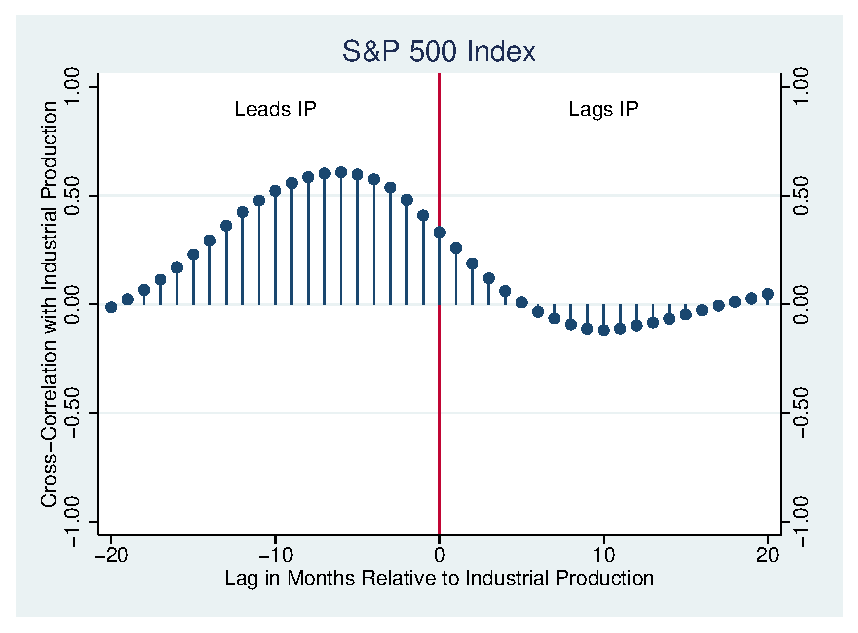
\includegraphics[scale=0.8]{xcsp500.eps}
    \caption{Cross-correlation function for 
    the S\&P 500 index and industrial production.
    The large correlations to the left tell us that 
    the S\&P 500 index is a good indicator of industrial production.
    Why?  Because the correlation is high (over 0.5) to the left
    (which indicates that the S\&P 500 ``leads'' industrial production).} 
    \label{fig:ccf-sp500}%
\end{figure}


Let's move from the abstract to the concrete to make sure we 
understand what the ccf represents.
[You might want to work your way through this paragraph slowly, 
it's important.]  
We calculate the year-on-year growth rates of the S\&P 500 index 
and industrial production and compute their ccf using 
the S\&P 500 for $x$ and industrial production for $y$.
Figure \ref{fig:ccf-sp500} is a plot of their correlations against 
the lag $k$.
There's a lot of information here, so let's go through it 
one dot at a time.
The dot at $k=0$ (on the vertical line at the center of the figure) 
shows that the contemporaneous correlation is about 0.2.
Contemporaneous means that we're looking at the two variables
at the same time:  
March 2001 industrial production is lined up with March 2001 S\&P 500, 
and so on.  
Next consider the dot corresponding to $ k = -10$ on the left
side of the figure.
The correlation of (roughly) 0.5 pictured in the figure 
shows the growth rate of industrial production with 
the growth rate of the S\&P 500 index dated 
10 months earlier.  
Evidently high growth in equity prices now 
is associated with high growth in IP 10 months later.
Finally, consider a dot on the right side of the figure.
The dot at $k=10$ suggests that the correlation
of industrial production growth with equity price growth 10 months
later is about --0.2.  

This pattern of correlations tells us a lot about the 
timing of movements in the two variables.  
In general, negative values of $k$ (the left side of the figure) 
indicate correlations of the S\&P 500 with
future industrial production; we would say they reflect the tendency 
of stock prices to lead output.
Positive values of $k$ (the right side of the figure) 
indicate correlations of the S\&P 500 with
past industrial production; they reflect 
the tendency of stock prices to lag output.  
What we see in the figure is a strong correlation of the S\&P 500 index
with industrial production 7-8 months later.
Evidently the stock price index is a leading indicator of 
industrial production.  

Let's look at some more indicators and see what they look like.
Some of the most common indicators are labor market variables, 
constructed by the Bureau of Labor Statistics.
Cross-correlation functions for four of them are pictured in 
Figure \ref{fig:ccf-labor}.
Nonfarm payroll employment (a measure of employment constructed 
from a survey of firm payrolls) is (apparently) a slightly
lagging indicator, since the ccf peaks with a lag of 1-2 months.
It is nevertheless useful, because the correlation (over 0.8) is 
unusually strong.
And even a 2-month lag is more timely than the GDP numbers.  
The unemployment rate is countercyclical (note the negative correlations) 
and lags IP in the sense that the largest correlation comes at a 
lag of 3-4 months.  
It seems that a rise in output is followed by a drop 
in the unemployment rate 3-4 months later.  
New applications (``claims'') for unemployment insurance 
are also countercylical, but the correlation is stronger than 
for the overall unemployment rate and it leads industrial 
production by 2-3 months.
Another popular labor market indicator is average hours worked per 
week in manufacturing.  
This indicator is strongly procyclical and leads industrial production
by 2-4 months.  
The labor market, in short, provides a good overall picture of the 
economy, and in some cases supplies 
indications of future movements in industrial production.
The leading variables (``new claims'' and ``average weekly hours'')
are more highly correlated with industrial production
than the S\&P 500 index, but the leads are shorter.  


\begin{figure}
    \centering
    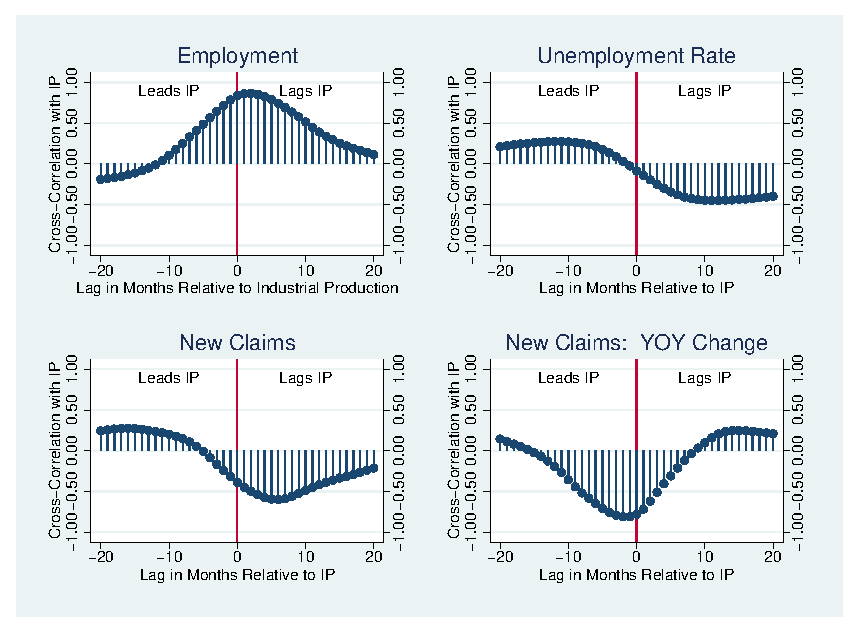
\includegraphics[scale=0.8]{xclabor.eps}
    \caption{Cross-correlation functions for 
    labor market indicators and industrial production.} 
    \label{fig:ccf-labor}%
\end{figure}

\begin{figure}
    \centering
    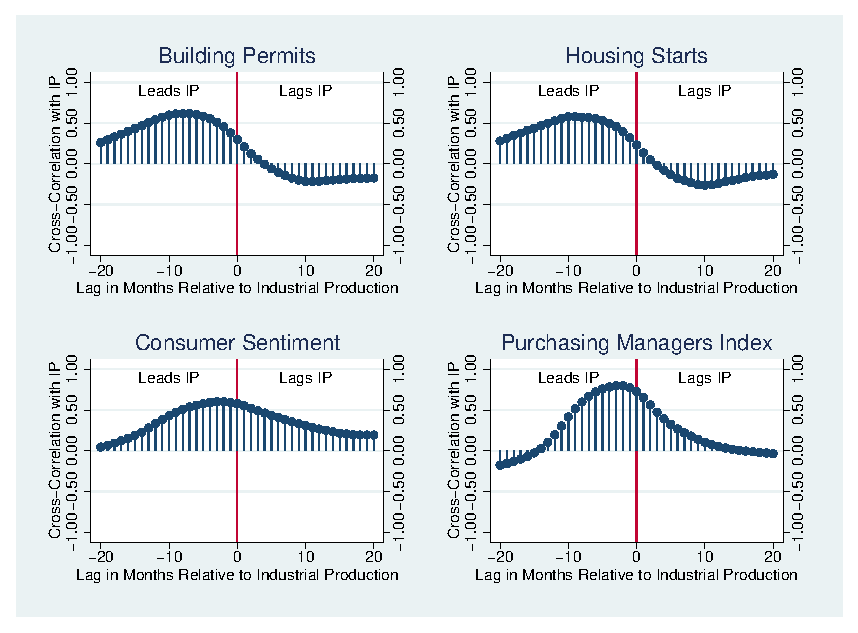
\includegraphics[scale=0.8]{xcsurvey.eps}
    \caption{Cross-correlation functions for 
    surveys of economic activity and industrial production.} 
    \label{fig:ccf-survey}%
\end{figure}

Another source of useful information are various measures and surveys 
of economic activity conducted by 
the Bureau of the Census and private organizations.
Cross-correlation functions for four common ones are pictured in 
Figure \ref{fig:ccf-survey}.
The first two are building permits and housing starts, 
two indicators of new home construction reported by the Census.
Two ideas lie behind their use:  that 
construction of new capital is more volatile than 
other sectors of the economy, 
and that decisions to build new homes reflect optimism 
about the future.  
The cross-correlation functions suggest they work:  
while the correlations are 
smaller than with (say) employment, the leads are substantial 
(10 months or so).  
The next two are popular private surveys.
Consumer sentiment is based on a survey of consumers 
collected by the University of Michigan.
It reflects consumers' optimism about current and future economic conditions.
The purchasing managers index is what we call a ``diffusion index.'' 
It's based on a survey of purchasing managers who report whether 
they see economic activity increasing or decreasing.  
The index reflects the shares of each.  
We see in the figure that both are procyclical leading indicators.


We could go on.  There are hundreds of indicators, more all the time.
The most common one we've skipped is the slope of the yield curve:
flat or downward-sloping yield curves are associated with slower-than-usual 
future growth in output.  
More on this in the Appendix. 



\subsubsection*{Regression-based forecasting}

Now that we have some indicators, how do we use them?  
Let's go through the steps we might follow in constructing a forecast 
of (say) industrial production $k$ months in the future.  


{\it 1. Decide what it is we're forecasting.\/} 
Let us say that we're interested in the growth rate of industrial 
production between now and $k$ months in the future.
You can do what you want, but we compute the (annualized) growth
rate this way:
\[
    \gamma_{t,t+k} \;=\; \log (\IP_{t+k}/\IP_t) \times (12/k) .
\]
We refer to $k$ (here measured in months) as the {\it forecast
horizon\/}.  The adjustment factor ``$12/k$'' converts the growth
rate to annual units.
For a one-year forecast, then, we would set $k=12$ and compute the 
year-on-year growth rate.  

{\it 2. Identify some good indicators.\/} 
The previous section might give you some ideas.
There's a half-step that sneaks in about here, too:
what form of the indicator to use.  
In most cases we use growth rates of the indicators, too, 
either over one period or a year, whichever you think works best.
But some variables are used as is.
In Figure \ref{fig:ccf-labor}, for example, 
cross-correlation for the unemployment rate for for the rate, period, 
not its growth rate, change, or other transformation.  

{\it 3. Run a regression.\/} 
Once we have a variable to forecast and some indicators, 
we use a statistical package to estimate a regression line
that links them.  
For example, to forecast IP growth, we would estimate the regression
\[
        \gamma_{t,t+k}  \;=\;  a + b x_t + \mbox{residual},
\]
where $x_t$ is the value of the indicator we have chosen.  
We use a sample of data to estimate the parameters $a$ and $b$.  
Note well:  the growth rate is between now (date $t$) 
and a future date ($t+k$), 
but the indicator is observed now (at $t$).  
This is central to the exercise:  we use what we know now 
to predict the future.
It's not kosher to use future variables to predict the future, 
because we don't know them when we make the forecast.  


{\it 4. Use the regression to compute a forecast.\/} 
Once we have estimates of the regression 
parameters ($\widehat{a}$ and $\widehat{b}$, say), 
we use them and the current value(s)  
of the indicator(s) ($x$, say) 
to compute the forecast: 
\[
        \widehat{\gamma}_{t,t+k}  \;=\;  \widehat{a} + \widehat{b} \; x_t .
\]
The ``hats'' remind us we are using estimates;
$\widehat{\gamma}_{t,t+k}$ is our forecast of future growth.  


There are lots of variants of this approach:
you can add multiple indicators, 
lags of the indicators  ($x_{t-1}, x_{t-2}, ...$), 
and even (esp?) past values of the growth rate of industrial 
production.
We recommend all of the above.  


Such exercises can generate useful forecasts --- 
useful in the sense that the forecast tells us something about the future.
But over periods of a year or two, 
the forecast accuracy is modest.
Even in-sample, the regressions rarely have $R^2$s above 0.25, 
which tells us that most of the future is unpredictable.
Some people see a lesson in this:  it might be more important
to know how to respond when the unexpected occurs
than to have better forecasts.   
In practice, both are useful:  knowing something about the future, 
and having backup plans to deal with the inevitable forecasting errors.  


\subsubsection*{Aggregation and prediction markets}

There's another appealing approach to forecasting:  
let markets do the work.  
Most of the best forecasts aggregate information from multiple
indicators and sources.  
Indexes of leading indicators do this one way:  they
combine various indicators to produce an index, which is then used
to forecast the future.  
Or we could use multiple indicators in regression-based forecasts, 
as we suggested above.  
Or we could aggregate the forecasts themselves.  
The so-called ``Blue Chip" forecast is an average of forecasts generated by experts, and it performs better, on average, than any single forecaster.  
Some statistical forecasters do the same sort of thing on their own:  
they generate multiple forecasts with methods like our forecasting regression,
then average them to generate a final aggregate forecast. Again,
the aggregate tends to do better than the individual forecasts.

A related idea is to rely on markets, which aggregate information
from a variety of sources.  Presidential futures markets, for
example, have predicted the popular vote in the last four
elections more accurately than any of the major polls.  
In the economic arena, there is a growing number of markets
in which you can trade futures contracts whose payoff is tied 
to the value of a particular economic number number:
the consumer price index, the fed funds rate, and so on.
These markets are increasingly used as forecasts themselves, with one wrinkle.
The simplest interpretation is that the futures price is a market forecast 
of the relevant economic number.  
For example, if we are interested in the value of an economic number $y$
to be released in 6 months ($y_{t+6}$, say), 
we might use it current future price ($f_t$, say): 
\[
    f_t  \;=\;  \mbox{Market's Current Expectation of  } y_{t+6} .
\]
Experience (and possibly some insight) tell us that we may want to make a
correction for the risk of the contract:  
\[
    f_t  \;=\;  \mbox{Market's Current Expectation of  } y_{t+6}  
                + \mbox{Risk Premium} .
\]
There's no limit to the amount of sophistication 
we can bring to bear on the last term, 
but for now you can simply note that 
we probably want to address it in some way.
Once you do, markets are an extremely useful source of information
about the future.  
An application to the yield curve is included in an (optional) 
appendix. 


\subsubsection*{Executive summary}

\begin{enumerate}
\item Fluctuations in economic activity can be (partially)
predicted by a number of indicators.  

\item The cross-correlation function is a tool for describing the 
timing of the statistical relation between two indicators:
whether, for example, one indicator leads another.    

\item We can generate forecasts with regressions that relate
future values of a variable of interest to the current value of
one or more indicators. 

\item Markets are useful aggregators of information ---  
and increasingly popular sources of economic forecasts.

\end{enumerate}


\subsubsection*{Review questions}

\begin{enumerate}

\item We mentioned building permits as a useful indicator 
of future economic activity. 
In what ways do you think it's a good indicator?  A bad one?  
Further information is available at the US Census Bureau's
\href{http://www.census.gov/const/www/newresconstindex.html}
{web site}.

Answer.  Good:  connected to housing, which as a durable good
should be cyclically sensitive and volatile; available quickly; it
leads the cycle (as you can see from its ccf). Bad: based on a sample,
which leads to short-term noise; revised periodically; 
housing is a small part of the economy.

\item In 2002, a government agency recommended that we establish a
futures market in terrorist attacks, on the grounds that it would
give us a useful public indicator of their likelihood.  The idea
was widely criticized.  Do you think it was a good idea or a bad
one?  What would you need to do to implement it?

Answer.  Another case of a good idea thrown out because it sounded
bad to politicians.  It's not clear such attacks are predictable,
but if they are we'd expect futures markets to do as well as any
other method.  To implement the idea, you'd need to define (and
possibly quantify) a terrorist event.

\item The term spread (a long yield minus a short yield) 
is strongly correlated with future output growth.  Why do you think that is?

Answer.  We've seen that a steep yield curve means that we expect
short-term interest rates to rise.  Short-term interest rates may
rise because the economy is growing quickly (interest rates are
typically higher in booms) and/or because we expect higher
inflation (sometimes associated with a booming economy).

\end{enumerate}


\subsubsection*{Further information}


There are many sources of leading indicators around the world
and lots of guides to them.
Among them:  
%
\begin{itemize}
%\item Richard Yamarone, 
%{\it The Trader's Guide to Economic Indicators\/}.  
%US only, pretty good overview.  

\item This is the best one I've seen:  
Bernard Baumohl, 
{\it The Secrets of Economic Indicators\/}.

\item The Conference Board, 
\href{http://www.conference-board.org/pdf_free/economics/bci/BCI-Handbook.pdf}
{\it Business Cycle Indicators Handbook\/}.

\item JP Morgan, 
\href{http://www.jpmorgan.com/pdfdoc/GlobalDataWatchHandbook.pdf}
{\it Global Data Watch Handbook\/};
good overview of indicators worldwide. 

\item Jim Stock and Mark Watson are the two leading academics working on 
economic indicators.  Their 2003 paper in the Richmond Fed {\it Economic Review\/}
is an interesting look back at the 2001 recession 
and why many didn't see it coming.  
Here's a 
\href{http://www.richmondfed.org/publications/economic_research/economic_quarterly/pdfs/summer2003/stockwatsonsummer03.pdf}
{link}.
\item The National Bureau of Economic Research 
runs an email alert service 
for major macroeconomic data releases, primarily for the US.  See 
\href{http://nber.org/releases/}{link}.

%\item Political Calculations' online recession calculator: 
%\href{http://politicalcalculations.blogspot.com/2006/04/reckoning-odds-of-recession.html}
%{link}.
%Uses the yield curve to compute the probability of a recession.  

\end{itemize}
%
All of this work requires some knowledge of statistics.  
If you'd like to learn more about forecasting economic and financial variables
specifically, we recommend the
course ``Forecasting Times Series Data'' (B90.2302), taught in alternate years by Professors Deo
and Hurvich, two of our best statisticians.


%\vfill \centerline{\it \copyright \ \number\year \  
%NYU Stern School of Business}


\newpage 
\subsection*{Appendix:  Reading the yield curve (optional)}

\bigskip
We describe how the yield curve can be used to infer
market expectations of future interest rates.
It's a concrete example of the kind of market-based forecasting
described in an earlier section.


\subsubsection*{The yield curve}

We use the yield curve to infer ``the
market's'' forecast of future short-term interest rates.  
Roughly speaking, the slope of
the yield curve tells us what the market expects of future
short-term interest rates. But before we explain how this works,
we need to review yields and forward rates.
Most of this should be familiar if you've taken 
``Foundations of Finance.''  

Yields and forward rates are subspecies of interest rates. {\it
Yields\/} are simply a way of reporting bond prices. If you go
into the bond business you'll find there are lots of details to
worry about (accrued interest, day count conventions, etc), but
we'll keep it simple and look at yields on bonds with no coupons
--- zero-coupon bonds or ``zeros.''  A one-year zero is a claim to (say) \$100 in
one year.  A two-year zero is a claim to \$100 in two years.  An
$m$-year zero is a claim to \$100 in $m$ years, and so on.  If the
price of an $m$-year bond is $p_m$, its yield $y_m$ is defined by
the present value formula:
\begin{equation}
        p_m  \;=\; 100/(1+y_m)^m.
        \label{eq:pv}
\end{equation}
This formula is based on annual compounding, which is the most
convenient convention for our purposes; more on this shortly. Note
that if we know prices, we can find yields, and vice versa. The
{\it yield curve\/} for zero-coupon bonds is a graph of yield
$y_m$ versus maturity $m$.


The yield curves you see in the newspaper are usually based on
yields of coupon bonds, and in the case of US treasuries they use
semi-annual compounding. They capture similar information, but
they're a little harder to make sense of.  Why?  Because the yield
depends not only on maturity, it also depends on the coupon. Since
the coupons vary over time and across maturities, it's never
exactly clear what we're talking about.  For that reason, most
formal fixed income analysis starts with prices and yields of
zeros.


{\em Example.} Suppose prices of zero-coupon bonds are
%
\begin{center}
\begin{tabular}{cc}
               Maturity        &     Price         \\
                1              &      94.24        \\
                2              &      87.70        \\
                3              &      81.22        \\
                4              &      75.16        \\
                5              &      69.66
\end{tabular}
\end{center}
%
What are the yields?

Answer.  The yields are 6.11, 6.78, 7.18, 7.40, and 7.50,
respectively, expressed as annual percentages.  The third one
solves the equation $ 81.22 = 100/(1+y_3)^3 $, namely $ 1 + y_3 =
(100/81.22)^{1/3} $.  The others are similar.



Yields are interest rates that apply over a number of periods. For
example, the $m$-year yield at date $t$ applies over the period of
time between $t$ (now) to $t+m$ ($m$ years from now).  One way to
think about the return on the bond is that the invests $p$ and
gets a rate of return equal to the yield $y$ for every period
until maturity.  In the two-period case, this leads to
\[
    100 \;=\; p_2 \times (1+y_2) (1+y_2) ,
\]
a variant of our present value formula, equation (\ref{eq:pv}).
Another way to think about the return is that the rates vary
across periods. In the two-period case, the bond might have
different rates of return in the first and second periods. But
what are these returns?  We know the return on a one-period bond
is $y_1$, so the first-period return should be $y_1$.  What about
the second period?  We need an interest rate that applies to the
second period alone but that remains consistent with the price of
the bond. That is, a rate $f_1$ that satisfies
\[
    100 \;=\; p_2 \times (1+y_1) (1+f_1) .
\]
Putting these two equations together tells us
\[
    (1+y_2)^2 \;=\; (1+y_1) (1+f_1)
\]
or
\[
    1+f_1 \;=\; p_1/p_2 .
\]
We refer to $f_1$ as the one-period-ahead {\it forward rate\/},
since it applies at date $t$ to the time period between $t+1$ and
$t+2$. It's the rate of return on a {\it forward contract\/} in
which we agree at $t$ to invest a fixed amount at $t+1$ for one
period.
For our purposes, you can think of forward contracts 
as identical to the more common futures.
The latter differ (a little) in having a mark-to-market requirement, 
which aficionados will take seriously but the rest of us can safely 
ignore.  

The same logic applies to bonds with maturities greater than two.
The bond price can be expressed as
\begin{eqnarray*}
        p_m &=& 100/(1+y_m)^m \\
            &=& 100/ [(1+y_1)(1+f_1) \cdots (1+f_{m-1})] .
\end{eqnarray*}
The two relations together imply
\begin{equation}
    1+f_{m-1} \;=\; p_{m-1}/p_{m} ,
    \label{eq:fdef}
\end{equation}
where $f_m$ is the $m$-period-ahead forward rate.  Draw a circle
around this equation: you'll be using it soon.  What we're doing
here is using bonds of two consecutive maturities to ``pick off''
the forward rate that applies over the last period.


Putting all the pieces together, we have three ways to express the
same information:  bond prices, yields, and forward rates. Given
data on a complete set of maturities, we can compute any one of
the three from any other.


{\it Example (continued).\/} For the bond prices and yields
reported earlier, verify that the forward rates are
%
\begin{center}
\begin{tabular}{cccc}
  Maturity ($m$)  &  Price ($p_m$)  &  Yield ($y_m$)  & Forward Rate ($f_{m-1}$) \\
     1      &  94.24  &   6.11 &   6.11    \\
     2      &  87.70  &   6.78 &   7.45         \\
     3      &  81.22  &   7.18 &   7.98     \\
     4      &  75.16  &   7.40 &   8.06       \\
     5      &  69.66  &   7.50 &   7.90
\end{tabular}
\end{center}
Note that the maturities of forward rates are one less than those
of bond prices and yields.  We do this because they naturally
start at zero, for reasons that may be clearer to you shortly. The
0-period-ahead forward rate is simply the current one-period
yield:   $f_0 = y_1$.

Answer.  We compute forward rates from prices.  For $m=5$, the
calculation implied by equation (\ref{eq:fdef}) is
\[
    1 + 0.0790 \;=\; 75.16/69.66.
\]
The others are similar.


\subsubsection*{Reading the yield curve}

Now that we've done all this work, we can use it to predict future
one-period yields.  Put simply but somewhat imprecisely, we're
going to say that forward rates are the market's expectation of
future one-period yields, plus an adjustment for risk that depends
on maturity but doesn't vary over time.  Once we've done the
adjustment, we can read expected future one-period yields from the
forward rate curve. The idea is referred to as the {\it
expectations hypothesis\/} because it's based on the premise that
forward rates include expectations of future one-period yields ---
{\it short rates\/} in conventional terminology.

To be more precise we need to add a little notation. Since we'll be dealing a lot with the
one-period yield or short rate, let us label it $i$, so that $i_t$ is the yield on a one-period
bond bought at date $t$. We label (one-period) forward rates by $f_{m,t}$, meaning the rate on a
forward contract arranged at date $t$ but applying to the period between dates $t+m$ and $t+m+1$.
The expectations hypothesis states that the forward rate is the market's expectation or forecast
of the future short rate plus a risk premium:
\begin{equation}
    f_{m,t} \;=\; E_t (i_{t+m}) + \mbox{risk premium}_m .
    \label{eq:eh}
\end{equation}
The risk premium is assumed to be constant across time but may
vary by maturity.  The notation $E_t$ is meant to convey the
expectation made at date $t$.  If we know forward rates and risk
premiums, we can compute expected future short rates.


That's what the expectations hypothesis is, but where does it come
from?  Let's think about what an investor would demand of a
forward rate.  An investor with a two-period time horizon has (at
least) two choices.  She could buy and hold a two-period bond at
date $t$, thus getting (according to our second interpretation)
returns of $ i_t $ in the first period and $ f_{1,t} $ in the
second.  Alternatively, she could roll over a one-period bond,
getting (again) $ i_t $ the first period and the short rate $
i_{t+1} $ in the second.  These two possibilities can be pictured
like this:
%
\begin{center}
\unitlength=0.6mm
\begin{picture}(100,50)
  \put(50,45){\makebox(0,0){Rollover Strategy}}
  \put(25,32){\makebox(0,0){$i_t$}}
  \put(75,32){\makebox(0,0){$i_{t+1}$}}
  \put(0,25){\line(100,0){100}}
  \put(0,25){\makebox(0,0){$ | $}}
  \put(50,25){\makebox(0,0){$ | $}}
  \put(100,25){\makebox(0,0){$ | $}}
  \put(25,18){\makebox(0,0){$i_t$}}
  \put(75,18){\makebox(0,0){$f_{1,t}$}}
  \put(50,5){\makebox(0,0){Buy and Hold Strategy}}
\end{picture}
\end{center}
%
If $ i_{t+1} $ were known, then we would expect the market to
drive the forward rate $ f_{1,t} $ and the future short rate $
i_{t+1} $ together:  $ f_{1,t} = i_{t+1} $. If the future short
rate were higher, then no one would buy the long bond.  Its price
would fall and the forward rate would rise.  If it were lower,
everyone would buy the long bond and bid up its price. In an
uncertain world, similar logic might lead us to guess that the
forward rate is the market's forecast of the future short rate,
with some adjustment for risk:
\[
    f_{1,t}   =  E_t ( i_{t+1} ) + \mbox{\em risk premium}   .
\]
Similar reasoning for longer maturities leads us to equation
(\ref{eq:eh}).


The only remaining issue is estimating the risk premiums.  There
are as many ways to do this as there are finance professors, but a
relatively simple method is to use the average difference between
the short rate and the $n$-period forward rate as an estimate of
its risk premium; that is, we use
\begin{equation}
    \mbox{risk premium}_m  \;=\; E (f_{m,t}  -  i_{t} )
\end{equation}
and estimate the expectation on the right with the mean. This
should work as long as forecast errors (the difference between the
future short rate and its expectation) are zero, on average, and
the distribution of the short rate doesn't change over time (the
means of the short rate and future short rate are the same).
Table~\ref{tab:meanrates} summarizes mean forward rates for US
treasuries for the period 1970-2000.  Since the short rate is the
first forward rate, we compute risk premiums by subtracting it
from the other forward rates.

\begin{table}[h]
\centering
\begin{tabular}{ccc}
\hline\hline
        Maturity   &    Mean Forward Rate   &  Risk Premium \\
\hline\hline
            1  &  7.51 &  0.00 \\
            2  &  8.10 &  0.59 \\
            3  &  8.39 &  0.88 \\
            4  &  8.57 &  1.06 \\
            5  &  8.67 &  1.16  \\
\hline\hline
\end{tabular}
\caption{Mean Forward Rates for US Treasuries, 1970-2000.}
\label{tab:meanrates}
\end{table}


{\it Example (continued again).\/} For the forward rates reported
earlier, what are the implied expected future short rates?

Answer.  The calculations are summarized by
%
\begin{center}
%\newlength{\oldtab}
%\setlength{\oldtab}{\tabcolsep} \setlength{\tabcolsep}{0.10in}
\begin{tabular}{cccc}
  Maturity ($m$) & Forward Rate ($f_{m-1}$) & Risk Premium & Future Short Rate ($i_{t+m-1}$) \\
     1      &   6.11       &    0.00      &    6.11 \\
     2      &   7.45       &    0.59      &    6.86  \\
     3      &   7.98       &    0.88      &    7.10  \\
     4      &   8.06       &    1.06      &    7.00  \\
     5      &   7.90       &    1.16      &    6.74
\end{tabular}
\end{center}
%\setlength{\tabcolsep}{\oldtab}
%

In short, we can read expected future short-term interest rates
from the forward rate curve, which we compute from the yield curve
for zeros.  If you find this interesting, there's a lot more on
related topics in the ``Debt Instruments'' course.

\vfill \centerline{\it \copyright \ \number\year \  NYU Stern
School of Business}

\end{document}
